\subsection{Quản lý phiên bỏ phiếu trên Redis}

Phiên bỏ phiếu (\textit{voting session}) là một loại dữ liệu tạm thời, được tạo ngay khi cử tri bắt đầu thao tác bỏ phiếu và tự hủy sau một khoảng thời gian ngắn. Mỗi phiên được lưu trên Redis dưới một khóa duy nhất gắn với định danh cử tri:

\begin{figure}[H]
    \centering
    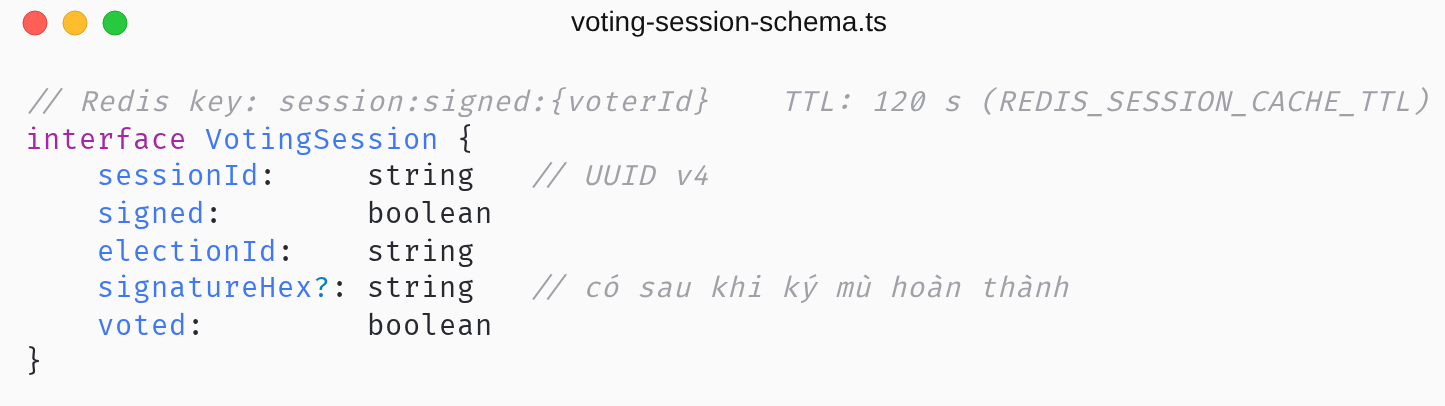
\includegraphics[width=0.65\textwidth, keepaspectratio]{Figures/code/voting-session-schema.png}
    \caption{Cấu trúc phiên bỏ phiếu lưu trên Redis và TTL 120 giây}
    \label{fig:voting-session-schema}
\end{figure}

Phiên hoạt động như một máy trạng thái phía máy chủ với ba trạng thái chính: \pkg{[start-session] $\rightarrow$ \{signed:\,false, voted:\,false\}} khi vừa khởi tạo, chuyển sang \pkg{\{signed:\,true, signatureHex\}} sau khi ba node ký phần đã hoàn thành ký mù, và cuối cùng chuyển sang \pkg{\{voted:\,true\}} sau khi phiếu được ghi nhận trên blockchain. Mỗi bước trong giao thức bỏ phiếu đều kiểm tra trạng thái phiên trước khi xử lý -- đảm bảo cử tri không thể bỏ qua các bước trung gian để gọi thẳng bước sau.

Khi cử tri khởi tạo phiên mới trong lúc phiên cũ chưa hoàn thành, hệ thống thực hiện hai thao tác đồng thời: ghi đè khóa cũ trên Redis bằng phiên mới, và phát sự kiện \pkg{DELETE\_SESSION\_NONCE} đến cả ba node ký để xóa nonce $k_i$ liên kết với phiên cũ trong bộ nhớ của chúng. Bước thứ hai là then chốt để chống tấn công khôi phục khóa do tái sử dụng nonce \textit{nonce reuse attack} -- nếu cùng một nonce $k_i$ được dùng để ký hai cặp $(r, s_i)$ khác nhau, kẻ tấn công có thể tính được khóa bí mật $d_i$ qua hai phương trình tuyến tính. Đoạn xử lý này trong \pkg{Coordinator} được trình bày trong Hình~\ref{fig:session-redis-delete-nonce}.

\begin{figure}[H]
    \centering
    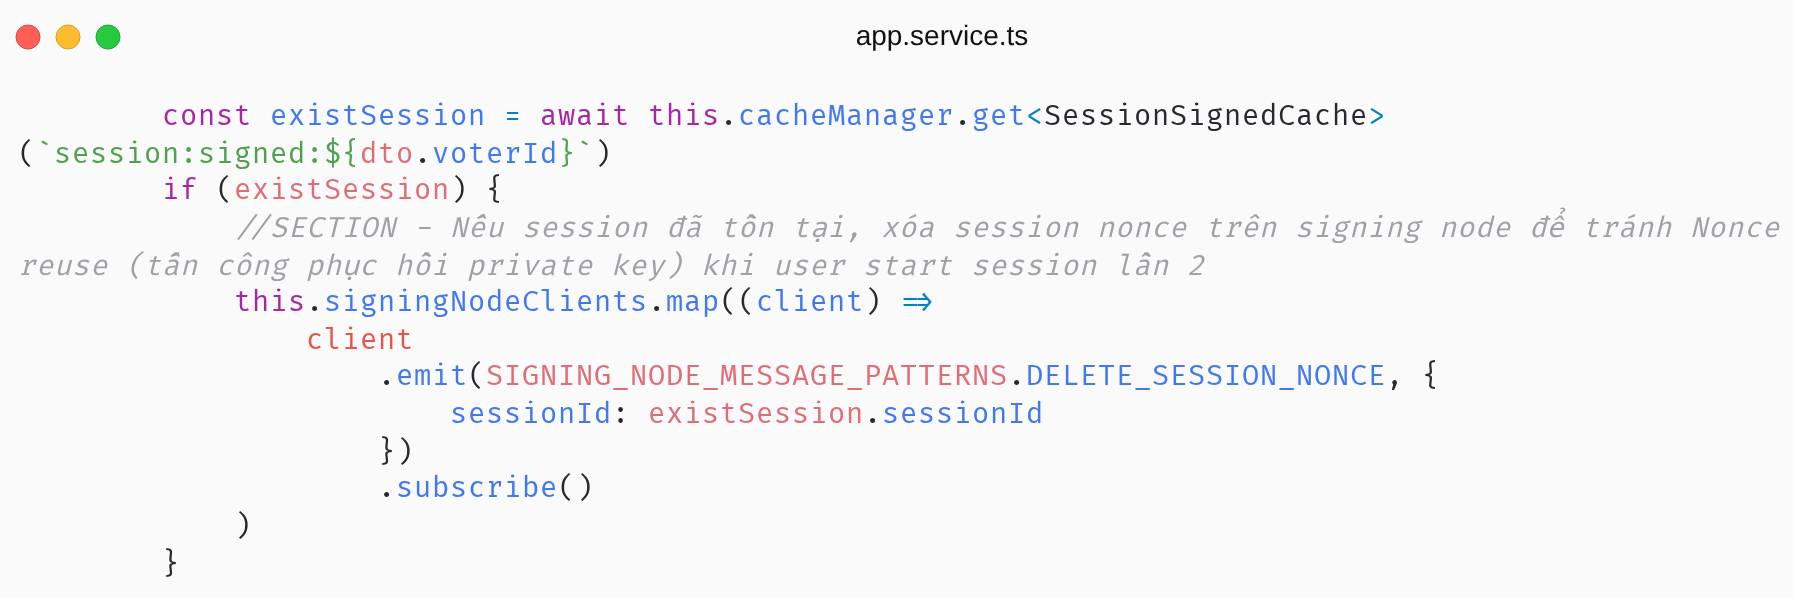
\includegraphics[width=0.85\textwidth, keepaspectratio]{Figures/code/session-redis-delete-nonce.png}
    \caption{Kiểm tra phiên cũ và phát sự kiện hủy nonce trước khi tạo phiên mới}
    \label{fig:session-redis-delete-nonce}
\end{figure}

Sau khi xóa nonce thành công, Coordinator tạo \pkg{sessionId} mới qua \pkg{uuidv4()}, gọi ba node ký để lấy cam kết và ghi phiên mới vào Redis với thời gian sống 120 giây (Hình~\ref{fig:session-redis-set}). Thời gian sống ngắn vừa đủ để cử tri hoàn thành quy trình bỏ phiếu (khởi tạo, ký mù, nộp phiếu), đồng thời đủ ngắn để phiên dở dang tự hết hạn và không chiếm bộ nhớ máy chủ. Khi thời gian sống của khóa Redis hết hạn, một cử tri muốn bỏ phiếu sẽ phải bắt đầu lại từ đầu -- cơ chế tự thanh lọc này tránh cho hệ thống phải lập lịch dọn dẹp riêng.

\begin{figure}[H]
    \centering
    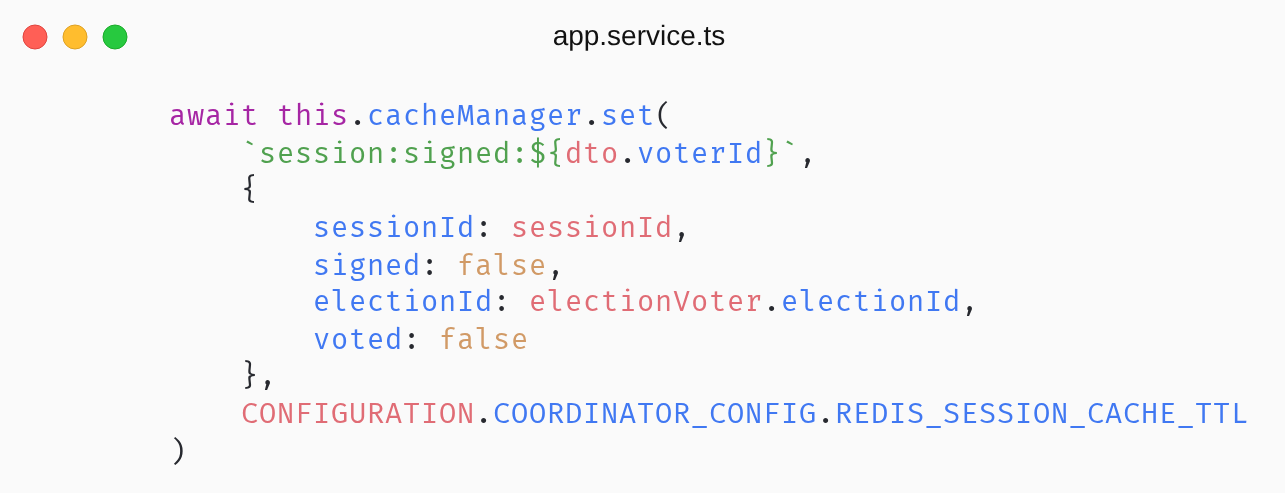
\includegraphics[width=0.85\textwidth, keepaspectratio]{Figures/code/session-redis-set.png}
    \caption{Ghi phiên bỏ phiếu vào Redis với thời gian sống 120 giây}
    \label{fig:session-redis-set}
\end{figure}
